\autsection{Salinity \& pH Sensor}{Kristian Sloth Lauszus and Lukas Christensen}

As previously noted, the pH and salinity of an environment is believed to play a large part in the formation of life. Therefore, sensors able to measure these quantities are an integral part of the instrument contingency of this mission. 

\subsection{Theory}
There exists multiple ways to perform electronic measurements of pH and salinity, however, most of them follow the same basic principle and are more or less variations of the Ion-Selective Electrode (ICE).\\

\noindent
The ICE works by having an electrode (the Ion-Selective Electrode) wrapped in a semi-permeable membrane submerged into the solution to be tested. The membrane is designed such that only ions of a single type, for example H$^+$, is able to penetrate it. When the chosen ion is present in the solution it will start to diffuse through membrane causing a build up of electrical potential across the it. In order to measure this potential difference another electrode, referred to as the reference electrode, is also placed into the solution as shown in figure \ref{fig:iseSchematic}. \\

\begin{figure}[htb]
	\centering
	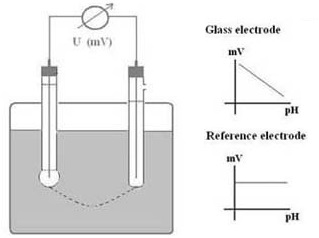
\includegraphics[width=.6\textwidth]{figures/LAMC/iseSchematic}
	\caption{Basic schematic of an Ion-Selective Electrode pH measurement setup. The left is the sensing electrode and the right is the reference. Adapted from \cite{website:ph2}.}
	\label{fig:iseSchematic}
\end{figure}

\noindent
By measuring the voltage across the electrodes the activity of the ion can be determined by the Nernst equation\cite{website:ph1}:
\begin{equation}\label{key}
E = E_0 + 2.303 \frac{R T}{n F} \log_{10}{(A)}
\end{equation}
Where $E$ is the measured potential, $E_0$ is a constant offset that depends on the exact construction of the two electrodes, $R$ is the universal gas constant, $T$ is the temperature, $n$ is the charge of ion to be measured, $F$ is the Faraday constant, and $A$ is the activity of the ion\cite{website:ph1}. As can be seen, the voltage varies linearly with the logarithm of $A$. This makes the ICE extremely well suited for pH-measurements, as the pH is directly proportional to the voltage, meaning only very simple data processing is needed.\\


\noindent
This seemingly simple setup is complicated by the fact that the reference electrode must be in electrical contact with the solution, without causing chemical reactions affecting the potential difference. The way this is most commonly accomplished is by having the reference electrode immersed in an electrolyte with a neutral pH that is separated from the solution to be measured by a membrane\cite{website:ph2}. A common issue with this is that the electrolyte will slowly leak out over time, meaning that the lifetime of an ICE is somewhat limited. \\

\begin{figure}[htb]
	\centering
	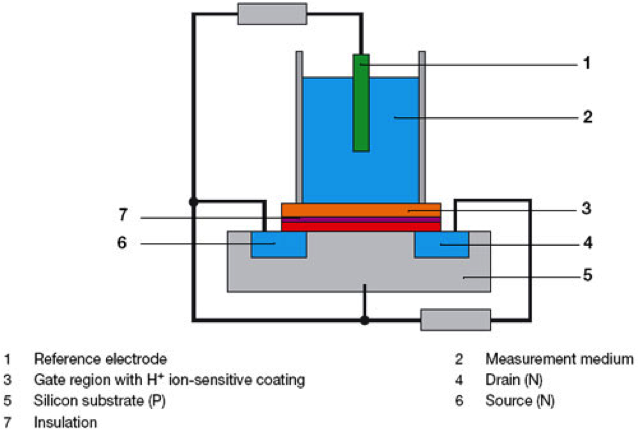
\includegraphics[width=.7\textwidth]{figures/ISFET.png}
	\caption{Schematic of an Ion-Selective Field Effect Transistor. Source: \url{http://www.jumo.de/products/liquid-analysis/ph/electrodes/201050/isfet-ph-single-rod-electrode-201050.html}}
	\label{fig:ISFET}
\end{figure}

\noindent
There are also a host of other issues associated with this type of measurements: To measure the potential difference, a very high impedance sensor is needed as the electrical resistance between the electrodes is commonly in the mega-ohm range\cite{website:ph3}. Furthermore, as can be seen from the Nernst equation, the temperature must be well known to make accurate measurements. Another issue is that the standard way to construct the ion-selective electrode is to have a metal conductor inside a glass bulb filled with an electrolyte, making the sensor fairly fragile. They also require frequent calibration and the membranes that are used to separate different ion-species are very difficult to construct in such a way that only one types of ion makes it through\cite{website:ph1}.\\

\noindent
The fragility and high impedance can be mitigated by the use of Ion-Selective Field Effect Transistors (ISFET). These consists of ordinary FETs but where the gate has been replaced with an ion-sensitive membrane as illustrated in figure \ref{fig:ISFET}. This means that if the sought-for ions are present in a sample that is brought to contact with the ISFET, it will start to conduct electricity proportional to the ion activity. The ISFET then acts as an amplifier and sensor simultaneously, simplifying the signal processing\cite{website:ph4}. Also, even though the membrane is made from a fragile material, such as glass, because only a small piece of it is needed for the gate, the ISFET can be made very durable with performances comparable to more classical methods\cite{website:ph4}. \\ 

\noindent
Other more exotic devices for pH and salinity measurement exist, such as for example voltammetry\cite{website:senova} and holography\cite{article:marshall2003a} based ones. While these devices show great promise and are able to overcome some of the issues associated with ICEs, they are still in their infancy compared to the extremely well characterized ICE systems. Because of this, as well as the fact that they have successfully been used in space before\cite{article:jgre2487}, the ICE provides a very robust solution.

\subsection{Implementation}
The initial sketch of the pH and salinity sensing system for this mission is inspired by the MECA Wet Chemistry Lab on the Phoenix Mars Scout Lander. The Phoenix mission used a number of ICE sensors with different membranes to measure pH and the abundance of various ions in Martian soil\cite{article:jgre2487}. The exact number and nature of the ions to be detected on Europa is beyond the scope of this report, as it would require experts with detailed knowledge in planetary physics and biochemistry in order to select the specific ions that will have the most scientific value. However, pH sensing shall no doubt be included, and the basic sensor design can easily be extended to host an almost arbitrary number of sub-sensors.

\subsection{Discussion}

It has been chosen, contrary to the Phoenix mission, to use ISFETs to form the basis of the sensing element. The reason for this is that these can be made very small, and since they are solid state devices they should easily be able to withstand the very high pressure that can be expected below the Europan ice sheet.\\

\noindent
Furthermore their exist sensors based on this techonology that requires no user calibration\cite{website:senova}. Which would simplify the instrument a lot. The sensors could simply be placed inside the penetrator having the water run by them similar to the approach described in \ref{sec:water_convection}, thus the pH and salinity could be measured contentiously during the entire descent with little effort and take up almost no volume and mass.
